\section{معیار‌های داده‌های چشمی و مغزی و ویژگی‌های آن‌ها}
\label{s:eye}
\subsection{مقدمه}
در بخش
\ref{s:CognitiveLoad}
دیدیم معیار های اندازه گیری شناختی را می‌توان به دو صورت دسته بندی نمود، نخست واقعیت گرانه 
\LTRfootnote{Objective}
و خود انگارانه یا مستقیم و غیرمستقیم. با این حال سنجش واقعیت گرایانه بارشناختی در میان پژوهش‌ها کمتر بوده‌ است. سنجش با فعالیت ثانویه که شامل یک فعالیت دیگر بودند و بار شناختی اعمال شده توسط فعالیت اصلی را با کارایی و یا زمان پاسخ فعالیت ثانویه اندازه‌گیری می‌شوند. سنجش با فعالیت ثانویه نمی‌تواند به صورت پیوسته بار شناختی را اندازه گیری نماید، با این‌حال می‌توان  زمان پاسخ دادن به فعالیت ثانویه را در بازه اعمال و یا نمایش محرک فعالیت ثانویه استناد نمود.
\cite{antonenko2010using}
\\
حال روش هایی مانند رهگیری چشمی و ای‌ای‌جی که در سال های گذشته عمدتاً در شرایط آزمایشی ویژه و محدود به کار می‌رفتند، اكنون به طور فزاینده در محيطهای یادگيری واقع گرایانه كاربرد دارد. قابليت این 
روشها برای پایش و سنجش آنی و كمی وضعيت شناختی و ذهنی یادگيرندگان، می‌تواند استفاده زیادی 
در بهينه سازی راهبردهای آموزشی داشته باشد.
\cite{jraidi2019assessing}
در این فصل، به بررسی سنجش بار شناختی با روش رهیاب چشمی در فرآیند یادگيری چندرسانهای از طریق فيلم آموزشی می‌پردازیم. 
همچنين جدیدترین پژوهشهای كاربردی این حوزه كه با كمک معيارهای چشمی به سنجش بار 
شناختی و یادگيری چندرسانه‌ای پرداخته‌اند، گزارش می‌كنيم.

سنجش پیوسته بارشناختی اجازه تحلیل دقیق تر میزان نوسان بارشناختی را با داشتن داده های زمان های مختلف به ما می‌دهد، بدین صورت می‌توان تحلیل و نتیجه‌گیری های دقیق تری از داده های بارشناختی و ارتباط آن با اثر انواع محرک های یادگیری داشت. روش های اندازه گیری واقعیت گرانه‌ی بار شناختی به ما این امکان را می‌دهند تا در تمامی سطوح شناختی شامل آنی، بیشینه، تجمعی، میانگین و سراسری بتوانیم بارشناختی را مورد بررسی قرار دهیم. از جمله این روش‌ها می‌توان به روش های سنجش  فیزیولوژیکی مانند: نرخ ضربان قلب
\LTRfootnote{Heart Rate Variability}
، حرکت چشم
\LTRfootnote{Eye Movements}
، سطح هرمون‌ها
\LTRfootnote{Hormone Levels}
و نوروآدرنالین
\LTRfootnote{Noradrenaline}.
و از جمله روش‌هایی که در علوم اعصاب استفاده شده‌اند، می‌توان به تصویرسازی تشدید مغناطیسی کارکردی (اف‌ام‌آرآی)
\LTRfootnote{Functional Magnetic Resonance Imaging(FMRI)}
، برش‌نگاری با گسیل پوزیترون (پِت اسکن)
\LTRfootnote{Positron Emission Tomography(PET)}
و نوار مغزی (ای‌ای‌جی)
\LTRfootnote{Electroencephalography(EEG)}
اشاره نمود.
\cite{antonenko2010using}
\\
به عنوان گزینه‌ای برای اندازه گیری بار شناختی هریک محدودیت های خود را نیز دارند، برخی ارتباط ضعیف تری با بار شناختی برقرار می‌کنند(مانند نرخ پلک زدن، مدت پلک زدن). روش سطح هرمون‌ها سرعت بسیار کمی دارد، نرخ ضربان قلب به نوسان‌های لحظه‌ای بار شناختی حساس نمی‌باشد. برخی اندازه گیری ها نیز بیش از حد دست و پا گیر و مزاحم هستند و یا نیاز به کاربر متخصص که به دو حیطه شناختی و پزشکی آشنا باشد دارند مانند پست اسکن و اف‌ام‌آرآی در این روش ها تصویر برداری عصبی با استفاده از پویش‌گرها و حس‌گرها تغییرها‌را در جریان خون مرتبط با فعالیت عصبی را ثبت می‌کنند. در یک پژوهش مشاهده شده است که انقباض مردمک که هیچ‌یک از این محدودیت‌ها را ندارد برای فعالیت هایی که شامل خواندن پیوسته باشد مناسب نیست. همچنین علائمی وجود دارد که پاسخ مردمک به تغییرهای بار شناختی بسته به سن شرکت کنندگان کاهش می‌یابد.
\cite{antonenko2010using}
\\
در شکل 
\ref{fig:neuromarketingtools}
می‌توانید روش های مختلف بررسی فعالیت های مغزی را مشاهده کنید.
\begin{figure}[htbp]
	\centering
	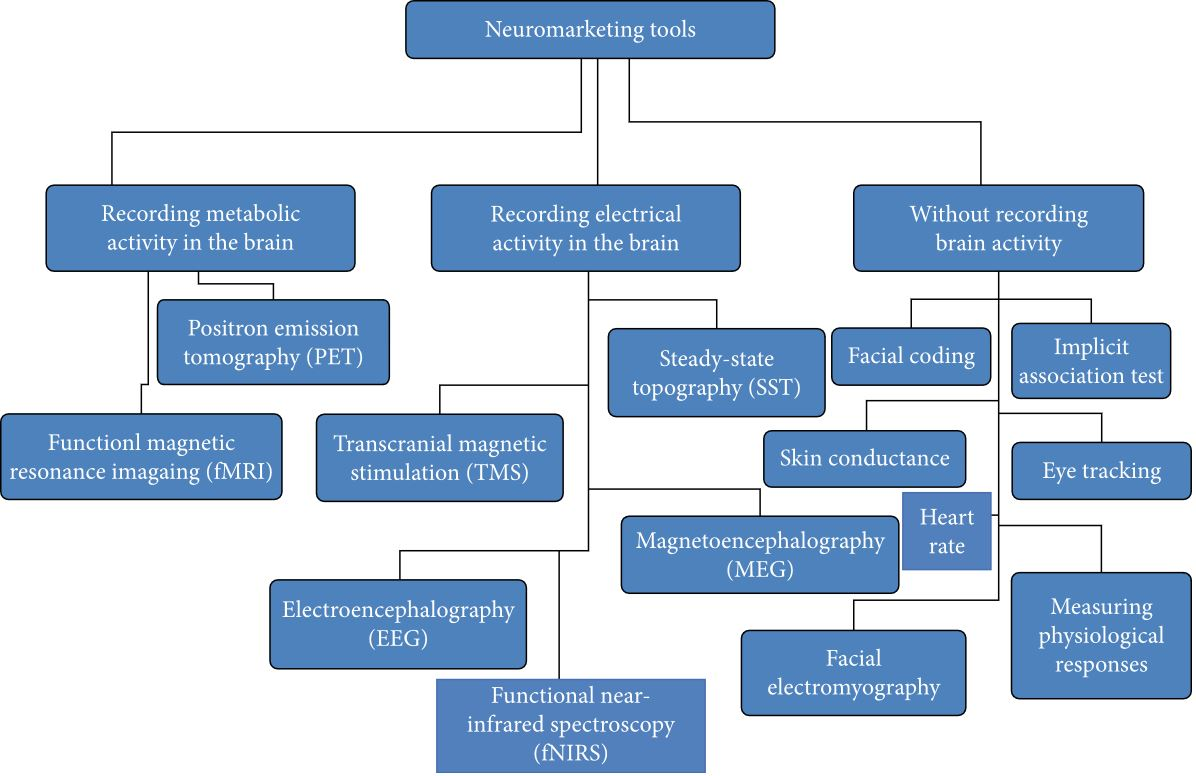
\includegraphics[width=\linewidth]{figures/Neuromarketing_tools}
	\caption[نمودار درختی روش‌های اندازه‌گیری بارشناختی]{نمودار درختی روش‌های اندازه گیری بارشناختی}
	\label{fig:neuromarketingtools}
\end{figure}


\subsection{پیشینه پژوهش های استفاده از ردیابی چشم}

نخست در سال ۱۸۷۹ لویس جوال مشاهده نمود که فرایند خواندن متن و حرکت چشم بر روی نوشته‌ها به صورت پیوسته و روان نیست، و در مکان های خاصی چشم متوقف (تثبیت چشم)و یا حرکت ناگهانی(پرش چشم) دارد.
با این مشاهده سوال های جالبی در قرن بیستم میلادی بررسی شدند،‌از جمله چشم بر روی چه کلمه‌‌هایی توقف می‌کند؟ ، به چه مدت؟ و چه زمانی چشم به کلمه ای که قبلا دیده است باز می‌گردد.
\\
نخستین دستگاه ردیابی چشمی توسط ادموند هوی ساخته شد، نوعی  لنز بود که با چشم در تماس بود و یک درچه برای مردمک چشم روی آن تعبیه شده بود. که این لنز به نشانه گر آلومنیومی کوچکی متصل بود، او با این دستگاه به بررسی بازگشت چشم بر روی کلمه‌ها پرداخت و نشان داد که چشم روی برخی کلمه توقف نمی‌کند.
اولین دستگاهی که مزاحمتی برای چشم ایجاد نمی‌کرد توسط گای توماس باس‌ول، ساخته شده، که پرتوهای نوری که به چشم تابیده می‌شد را بر روی فیلم ذخیره می‌نمود. آلفرد یاربوس در کتابی که در ۱۹۶۷ میلادی منتشر کرد پژوهش های مهمی را بیان کرد و به طور خاص به رابطه تثبیت چشم و علاقه پرداخته بود.
در طول دهه ۱۹۸۰ جاست و کارپنتر فرضیه مهمی را بیان کردند که می‌گفت هر جا که چشم بر روی آن متوقف شده است ما در حال فکر کردن به آن هستیم و هرچه مدت زمان تثبیت بیشتر باشد بار شناختی بیشتری ایجاد شده است.
همچنین آغاز پاسخ دهی به سوال های رابطه انسان-رایانه بود.
در پژوهش های اخیر به رابطه میان انسان و کامپیوتر و استفاده از چشم برای تهسیل آن و آنالیز صفحه‌های وب پرداخته شده.
\\
به گفته هفامن توجه بینایی همیشه در حدود ۱۰۰ تا ۲۵۰ میلی ثانیه جلو تر از حرکت چشم قرار دارد و هر جا که توجه بینایی ما می‌رود چشم هم دنبال می‌کند.
\cite{deubel1996saccade}
به لطف پیشرفت فناوری و علم اکنون ردیابی های چشمی همراهی که بر روی چشم استفاده می‌شوند ساخته و تجاری سازی شده است، و دانش شبکه های عصبی عمیق
\LTRfootnote{Deep Learning Neural Network}
به ما کمک می‌کند تا بتوانیم این داده های چشمی را بهتر از گذشته پردازش کنیم.
\cite{wiki:EYET}
\subsection{مزیت‌ها و محدودیت‌ها‌ی اندازه گیری بار شناختی با استفاده از رهیاب چشمی}
\label{ss:ProVsCon}

برخلاف سایر دستگاههای فیزیولوژیکی که نیازمند دراز کشیدن شخص‌ در وضعیت محصور است (اف‌ام‌آرآی) یا خوردن مواد خطرناک(پِت‌اسکن)، ای‌ای‌جی بدون ورود به بدن می‌تواند فعالیتهای مغزی را به‌صورت‌ معتبر و با تنظیم‌های دنیای واقعی
\LTRfootnote{Real-World}
اندازه‌گیری کند.
\\
پیش از این فعالیت های مغزی با روش هایی چون نوار مغزی و مگنتوانسفالوگرافی یا به اختصار MEG
\LTRfootnote{Magnetoencephalography}
تهیه می‌شد. هدف این گونه ابزار ها رصد تغییر‌های میدان های مغناطیسی ایجاد شده در جمجمه توسط تغییر‌های جریان در نورون های مغزی بود.
بار شناختی یکی از شاخصه های فعالیت مغز است. عمده محبوبیت این روش ها دقت آن‌ها در حدود میلی ثانیه است، با اینحال عموما تنظیم آن آسان نیست و محاسبه‌های آن پیچیده تر است. همچنین نمی‌توان از داده های آن به صورت همزمان استفاده نمود و محل استفاده از آنها نمی‌تواند مکان های عمومی و یا حتی در مکان های عادی باشد.
\\
روش های بسیار غیر نورونی دیگری وجود دارد که نشان دهنده فعالیت های مغز و بار شناختی است. فعالیت های قشر بیرونی مغز سبب ایجاد تغییرهایی در ضربان قلب، فشار خون، الکترودرمال یا به اختصار EDA
\LTRfootnote{Electrodermal Activity}
، فعالیت های الکتریکی در عضله‌‌های صورت، حرکت‌های چشم و گشودگی مردک چشم.
\\
پژوهش های اخیر بر روی حرکت مردمک چشم جهت اندازه گیری بار شناختی سرمایه گذاری کرده‌اند.
تا کنون پژوهش های زیادی بر رابطه‌ی بین حرکت‌های ارادی چشم مانند توقف یا تثبیت چشم و پرش چشم با بارشناختی و یا حرک‌ت‌های غیر ارادی مثل پلک زدن و گشادی مردمک. به این حرکت‌های چشم رفتاری(ارادی) و فیزیکی(غیر ارادی) نیز گفته می‌شود.
با دنبال کردن حرکت‌های چشمی می‌توان به بررسی واکنش فیزیکی افراد نسبت به آزمایش  و سیستم می‌توان واسط کاربری متناسب با آن طراحی نمود.
به عنوان مثال در شرایط کنترل شده، رهیاب های چشمی با دقت بالا و مردمک سنج‌ها می‌توانند برای شناسایی کوچکترین گشودگی در مردمک استفاده شوند که نشانه بار شناختی است.
\cite{rafiqi2015pupilware}
با این حال باید توجه شود که سیستم های نمایش اطلاعات محتوی های بسیاری را نشان می‌دهند، نمایش اطلاعات و تعامل کاربر با سیستم تنوع بسیاری دارند که این خود سبب سخت شدن در استفاده مستقیم از حرکت‌های چشم در سنجش بار شناختی در مکان های عادی می‌شود. از این رو مهم است که رابطی بین حرکت‌های چشم و بار شناختی پیدا شود.
\cite{zagermann2016measuring}
\\
\textbf{تعامل انسان و رایانه}
\LTRfootnote{human computer interaction - HCI}
 به دانش و فناوری مدرن و پرتنوع مطالعه، طراحی، اجراء، و ارزیابی سامانه‌های محاسباتی درگیر در محاوره‌ها و تعامل‌های مابین کاربران انسانی از یک سو، و رایانه‌ها و عامل‌های هوشمند نرم‌افزاری از سوی دیگر گفته می‌شود. این دانش به بررسی تعامل انسان و رایانه می‌پردازد، در واقع نقطه تقاطع علوم رایانه و علوم رفتار‌شناسی طراحی است.

ما باور داریم جنبه‌هایی از تعامل کامپیوتر با انسان
، می‌تواند به ما کمک کند بهتر تاثیر کار با کامپیوتر را بر  حرکت‌های چشم بفهمیم، مخصوصا اگر داده های فروانی برای بررسی موجود باشد.
تعامل انسان با کامپیوتر عامل مهمی است چون: تعامل به شما امکان می دهد محدودیت ها را از نظر انسانی یا طرف محاسباتی مدیریت کنید مثلا با نمایش اطلاعات با سطح متفاوتی از جزئیات جابه‌جایی بین پنجره ها و نمایش های مختلف اطلاعات در نتیجه رشته تعامل انسان و رایانه نظریه هایی را فراهم می‌کند که واسط های کاربری‌ای طراحی شوند که به عامل های انسانی و قدرت پردازش رایانه بپردازند.
\\
در کنار همه اینها اکثر سیستم های امروزی به دوربین مجهز می‌باشند که می‌تواند چهره را رهیابی کند، در نتیجه استاندارد کردن رهیاب چشمی با همین پیاده سازی زیاد سخت نخواهد بود. اگر ارتباطی میان شناخت و حرکت‌های چشم باشد،‌ این اطلاعات می‌تواند کمک کند تا سیستم خودش را بار شناختی شخص مطابقت دهد.
در جدول 
\ref{tab:eye-procon}
به طور خلاصه می‌توانید نقاط قوت و ضعف اندازه گیری بار شناختی با استفاده از ردیابی چشمی را مشاهده نمایید.

\begin{table}[]
	\caption{مزایا و معایب داده‌های چشمی}
	\label{tab:eye-procon}
	\begin{tabular}{|c|c|}
		\hline
		مزایا                                                                                                             & معایب                                                                                                                              \\ \hline
		\begin{tabular}[c]{@{}c@{}}اندازه گیری بار شناختی\\ به صورت همزمان\end{tabular}                                   & \begin{tabular}[c]{@{}c@{}}هنگامی که چیزی نمایش داده نشود\\  مثلا هنگام استراحت،\\  اطلاعی از بار شناختی کاربر نداریم\end{tabular} \\ \hline
		\begin{tabular}[c]{@{}c@{}}با یک حسگیر می‌توان سه سیگنال حرکت‌های چشم،\\ تغییرات مردمک و پلک زدن را گرفت\end{tabular} & \begin{tabular}[c]{@{}c@{}}با عوض شدن سریع عکس\\  و شدت روشنایی مردمک\\  تحت تاثیر قرار می‌گیرد\end{tabular}                       \\ \hline
		می‌توان درهرجایی داده‌های چشمی گرفت                                                                                &                                                                                                                                    \\ \hline
		\begin{tabular}[c]{@{}c@{}}نشان داده شده که در آزمایش های تصویری \\ و صوتی با بار شناختی مرتبط است\end{tabular}   &                                                                                                                                    \\ \hline
		\begin{tabular}[c]{@{}c@{}}داده ها از راه دور گرفته می‌شوند \\ و کاربر کمترین اذیتی نمی‌شود\end{tabular}          &                                                                                                                                    \\ \hline
	\end{tabular}
\end{table}

\subsection{دستگاه ردیاب چشمی}
دستگاه های ردیاب چشم به ما کمک می‌کنند تا انواع حرکت‌های چشم را اندازه گیری کنیم.
به طور خلاصه می‌توان گفت دستگاه های ردیاب چشمی در این سه دسته قرار دارند: دستگاه ردیاب متصل به چشم، ردیابی نوری و اندازه‌گیری از طریق پتانسیل الکتریکی. در تصویر
\ref{fig:eyetech}
روش های مختلف ردیابی چشم را می‌بینید.

\begin{figure}[htbp]
	\centering
	
	\begin{subfigure}{.8\textwidth}
		\centering
		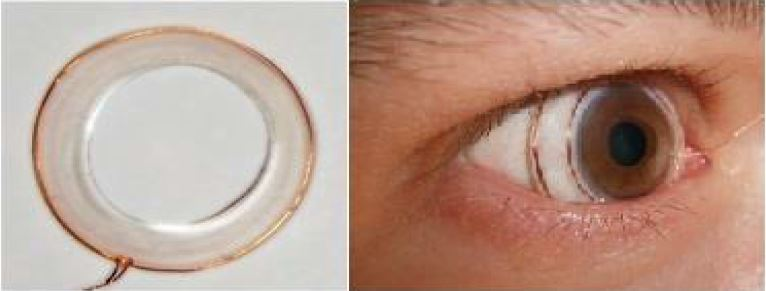
\includegraphics[width=0.7\linewidth]{figures/contact_lens}
		\caption{ردیابی چشم به وسیله لنز تماسی}
	\end{subfigure}
	\newline
	\begin{subfigure}{.8\textwidth}
		\centering
		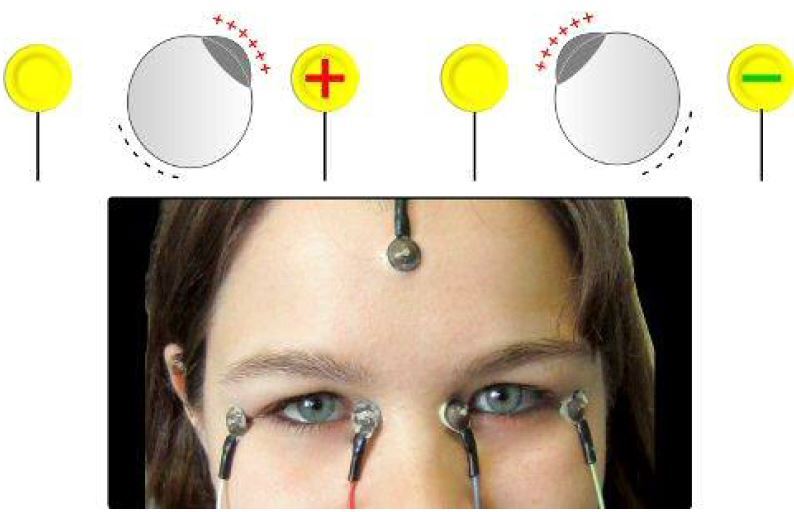
\includegraphics[width=0.7\linewidth]{figures/EOG}
		\caption{ردیابی چشم به وسیله بار الکتریکی}
	\end{subfigure}	
	\newline
	\begin{subfigure}{.8\textwidth}
		\centering
		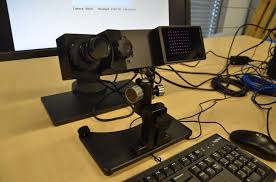
\includegraphics[width=0.7\linewidth]{figures/optical}
		\caption{ردیابی چشم با دوربین های نوری}
	\end{subfigure}

	\caption[ابزار های مختلف ردیابی چشم]{ابزار های مختلف ردیابی چشم}
	\label{fig:eyetech}
\end{figure}



\subsection{معیار‌های رهگیری چشم}
\label{ss:EyeMeasure}
اندازه‌گيری‌های فيزیولوژیک كه در دسته‌ی روشهای واقع‌گرایانه سنجش بار شناختی جای می‌گيرند،
ابزارهای مناسبی برای درک ارتباط بين حافظه‌ی كاری و یادگيری هستند. اغلب این اندازه‌گيری‌ها، امکان 
ثبت لحظه‌ای بار شناختی را فراهم می‌كنند .یکی از پركاربردترین این روشها، رهگيری چشمی است. 
داده‌هایی كه توسط دستگاه ردیاب چشم 
\LTRfootnote{Eye-tracker}
جمع‌آوری می‌شود در تحليل بسياری از فعاليت‌های شناختی
مورد استفاده قرار می‌گيرد.
\\
معيارهای مختلفی از داده‌های استخراج شده توسط دستگاه ردیاب چشم مورداستفاده قرار می‌گيرند،
برای مثال مدت زمان تثبيت چشم و نرخ پلک زدن در پژوهش‌های بسياری برای ارزیابی بار شناختی به كار 
رفته‌اند. برخی از این معيارها، ناشی از حركات ارادی چشم هستند و برخی غيرارادی اند. در ادامه، هر یک 
از این معيارها معرفی  خواهد  شد  و  ارتباط  هریک با  بار  شناختی بر  اساس  پژوهش‌های گذشته  بيان
می‌شود.
\\
حرکت چشم، شامل هر نوع حرکت ارادی و یا غیر ارادی برای پیدا کردن، تمرکز و دنبال کردن محرک های چشمی می‌گویند.

\subsubsection{تثبیت چشم}
رایج ترین رخدادی که در دستگاه رهیاب چشمی رخ می‌دهد، زمانی است که شخص در حالت تمرکز باشد و چشم ها در یک مدت زمانی ثابت باشند به این رویداد تثبیت چشم
\LTRfootnote{Fixations}
گویند. مدت آن از ۲۰۰ الی ۳۰۰ میلی‌ثانیه تا چند ثانیه خواهد بود و زاویه‌ای حدود 
$^\circ$۱
 است. این یک رویداد ارادی است. تعداد تثبیت ها نشان دهنده تعداد دفعاتی است که یک کابر به مکان خاص
\LTRfootnote{area of interest (AOI)}
نگاه کرده است.
پس حالت توجه با مکان خیره شدن در صحفه و یا مکان خاص مشخص می‌شود.
\\
رادمن و همکاران 
\cite{rudmann2003eyetracking}
متوجه شدند جهت خیره شدن نشان دهنده علت بار شناختی فعلی است. همچنین می‌توان از زمان تثبیت و یا خیرگی
\LTRfootnote{fixation duration}
به عنوان عامل نشان دهنده سطح بار شناختی استفاده نمود. این عمل با کاهش نرخ تثبیت همراه خواهد بود. چن و همکاران نشان دادند نرخ و زمان تثبیت با پیچیدگی آزمایش افزایش پیدا می‌کند.

\subsubsection{پرش چشم}

پرش چشم
\LTRfootnote{Saccades}
اشاره به حالتی دارد که که چشم بین دو موقعیت جابه‌جا می‌شود.
پرش چشم و خیرگی می‌توانند با استفاده از الگوریتم هایی که مکان طولی و عرضی مردمک را پردازش می‌کنند به صورت خودکار از یکدگیر جدا و برچسب گذاری‌ شوند.
به صورت ارادی است و پس از تثبیت رخ می‌دهد.
تثبیت و پرش چشم توسط سیگنالهای عصبی از سیستمهای قشر مغز و تحت قشر رمزگذاری می شود. این حرکت سریع ترین حرکتی است که بدن می‌تواند انجام دهد وبین ۳۰ تا ۸۰ میلی ثانیه طول می‌کشد تا انجام شود. رایج‌ترین شیوده تجسم پرش چشم، مسیرهای پویش
\LTRfootnote{Scanpath}
است. 
 می‌توان سرعت و طول پرش چشم‌ها را 
سنجيد و الگوهای مسير پویش را مشاهده كرد.
\cite{zagermann2016measuring}
چن و همکارانش، از اندازه‌گيری سرعت پرش چشم و 
طول آن به منظور بررسی تلاش ذهنی انسان استفاده كردند. نتایج آنها نشان داد كه سرعت و طول پرش 
چشم مولفه‌هایی  تفکيک  كننده  برای  دستیابی  به  كارآیی بالا  هستند.
\cite{chen2011eye}
همچنين،  مانوئل  و 
همکارانش دریافتند كه كاهش سرعت پرش چشم نشان دهنده خستگی و افزایش آن نمایان‌گر افزایش 
سختی كار است.
\cite{barrios2004adele}
بر اساس این یافته‌ها، بار شناختی با سرعت و طول پرش چشم نسبت مستقيم 
دارد؛ یعنی افزایش این دو شاخص، نشان دهنده افزایش بار شناختی است.
\paragraph{دامنه پرش}
یک ویژگی مفید دیگر، دامنه پرش
\LTRfootnote{Saccade Amplitude}
است، که اشاره به سختی دنبال کردن و یافتن دقیق مکان هدف مورد نظر دارد.
\cite{Hyona2003}
\subsubsection{گشادی قطر مردمک}
یکی دیگر از معيارهای چشمی گشاد شدن مردمک چشم
\LTRfootnote{Pupil dilation}
است،
عملکرد اصلی تغییر قطر مردمک محافظت از شبکیه (در برابر تابش نور) است و همچنین برای پاسخ به تغییر در تثبیت تصویر و واضح کردن آن برای اشیاء دور تا نزدیک.
تغییراتی که بازتاب تغییرات در فعالیتهای شناختی است در مقایسه با تغییرات ناشی از بازتاب نور و انعکاس اشیا نزدیک ، نسبتاً اندک است و علاوه بر آن تغییر در نور نسبتا سریع تر تغیرات مردمکی را در بر خواهد داشت.
بنابراین ، اگر اشیاء دارای عمق تقریباً ثابت در قسمت دیداری کاربر (بیمار) باشند، ما می‌توانیم داده های فرکانس پایین مردمک را استفاده کنیم.
\\
پس از دهه‌ها بررسی و مطالعه تغییرات مردمک هنوز محققان در منشا آن توافق ندارند، عده‌ای بر این باورند که منشا آن فشار ذهنی است و گروه دیگر برانگیختگی عاطفی را دلیل این تغییرات می‌دانند.
مشاهدات تجربی نشان می‌دهند مردمک در مواجه با تصاویر و صداهای بیشتر برانگیخته‌تر می‌شود، صرف نظر از بار احساسی ذاتی آن.
یک پژوهش اولیه روی بار احساسی و شناختی سعی بر ثابت نگه داشتن بارشناختی و ترکیب چند بار شناختی نمود نتیجه آن بود که بار شناختی تغییرات بیشتری در مردمک چشم ایجاد می‌کند.
\cite{Chen2013}
 پاسخ مردمک به عنوان یک واكنش غيرارادی رخ می‌دهد.
گشادی مردمک یک سیگنال فیزیولوژیکی است که که تغییراتش بسته به فعالیت های خودکار سیستم عصبی در دستگاه عصبی پیرامونی است.
قطر مردمک چشم می‌تواند بين  1/5 تا 8 ميلیمتر تغيير كند. روان‌شناسان در بيش از دو دهه اخير، تاكيد دارند 
تغييرات قطر مردمک، پردازش شناختی پرتلاشی را همراه دارد. پژوهش‌های گذشته نشان می‌دهند كه 
مردمک  بيننده  هنگامی  كه  سختی  كار  و  تلاش  شناختی  فرد  برای  پاسخ  به  آن  افزایش  می‌یابد،  گشاد 
می‌شود. مطالعه‌های زیادی اعتبار این استدلال را در كارهای مختلفی شامل مطالعه، حل مسئله و كارهای
دیداری تایيد كردهاند.
\cite{zagermann2016measuring}
همچنين پورتا و همکارانش، كاهش اندازه قطر مردمک در آستانه‌ی پایان كار در  آزمایش  خود  را  به  عنوان  نشانه‌ای  نهفته  برای  خستگی  قلمداد  كرده‌اند.
\cite{porta2012emotional}
علاوه  بر  فرآیندهای شناختی، تغييرات  در  روشنایی  محيط  تغييرات  در  اندازه  قطر  مردمک  را  در  پی  دارد.  با  تاریکتر  شدن محيط،  مردمک  چشم  برای  كسب  نور  بيشتر  گشاد  و  با  روشنایی  بيشتر  محيط، تنگ  می‌شود.  كنترل 
روشنایی محيط و درخشندگی نمایشگر یک چالش جدی در شرایط آزمایشگاهی است كه تغييرات در قطر مردمک  را  مطالعه  می‌كند.
\cite{zagermann2016measuring}
به  این ترتيب، افزایش  بار شناختی  باعث  گشادی مردمک چشم خواهد شد.
\subsubsection{پلک زدن}
چشم‌ما با هدف کاربری ۲ تا ۴ بار در دقیقه پلک می‌زند. اهداف غیر کاربردی دیگری مثل پلک‌زدن انعکاسی(یک پاسخ محافظ، مثل نزدیک شدن ناگهانی اشیا به سمت چشم)،‌ پلک‌زدن ارادی، پلک زدن درونی(غیر آگاهانه رخ‌ می‌دهد) و بسیاری از پلک‌زدن های ما از این نوع است که توسط سیستم عصبی مرکزی کنترل می‌شود و با شناخت ما ارتباط دارد. در نتیجه این نوع از پلک زدن ها برای اندازه گیری بار شناختی استفاده می‌شود.
\\
یک یافته نشان می‌دهد با افزایش تمرکز برای دریافت اطلاعات بیشتر از محرک نرخ پلک زدن کاهش می‌یابد دیدگاه دیگری در مقابل بیان می‌کند که پلک زدن مکانیزمی جهت آزادسازی و آسودگی است به طور مثال در هنگامی که به چیزی فکر نمی‌کنید و یا پایان آزمایش به ندرت پلک می‌زنید زیرا فشار ذهنی در هنگام حل مسئله بوده است. هنگامی که فشار ذهنی نتواند نمود درونی یا بیرونی پیدا کنید میزان پلک زدن افزایش می‌یابد.
باید سعی کنیم از طولانی بودن پنجره زمانی پلک زدن مطمئن شویم تا بتوان تغییرات محسوسی در هنگام اجرای آزمایش پیدا نمود.
\cite{Chen2013}

نرخ و تأخير در پلک زدن 
\LTRfootnote{Blink rate}
می‌تواند یک معيار رهگيری چشم دیگر در ارتباط با بار شناختی باشد.حرکت پلک‌ها توسط دستگاه عسبی مرکزی
\LTRfootnote{central nervous system (CNS)}
کنترل می‌شود.
 پلک زدن،  هرچند  می‌تواند  ارادی  هم  باشد،  یک  حركت  غيرارادی  در  نظر  گرفته  می‌شود.  نرخ  و  تأخير  پلک زدن‌ها، می‌تواند در فهم عميق درباره حالت توجه بيننده كمک كند.
\cite{zagermann2016measuring}
به عنوان مثال، تأخير زیاد و نرخ 
كم  پلک  زدن  به  عنوان  شاخصی  برای  تلاش  ذهنی  زیاد  دانسته  شده  است.
\cite{chen2011eye}
همچنين  مانوئل  و 
همکارانش، دریافتند كه افزایش نرخ پلک زدن و كاهش سرعت آن و نيز كاهش ميزان باز بودن پلکها، 
نشانه‌هایی برای افزایش خستگی هستند.
\cite{barrios2004adele}
بر اساس این یافته‌ها، می‌توان گفت: افزایش بارشناختی 
با كاهش نرخ پلک زدن و افزایش تأخير در پلک زدن نسبت مستقيم دارد. همچنين ممکن است بين بار 
شناختی و سرعت پلک زدن نيز رابطه‌ای وجود داشته باشد.
\subsubsection{ریزپرش چشم}
ریز پرش چشم
\LTRfootnote{Microsaccade}
یکی دیگر از حرکت‌های چشم است که توسط دستگاه ردیاب چشمی اندازه‌گیری می‌شود. ریزپرش‌‌ها غیر ارادی هستند همانند پرش‌ با دامنه کم هستند و در حالتی که چشم سعی در تثبیت دارد رخ می‌دهند.
\cite{Krejtz2018}
از جمله ویژگی‌های مثبت این معیار می‌توان به عدم حساسیت به میزان نور محیط اشاره کرد و دیگر آن‌ که با توجه به واکنش سریع و حساسیت این نوع حرکت می‌توان آن را در اندازه‌گیری بارشناختی به صورت همزمان استفاده نمود. 

\subsubsection{دنبال کردن روان}
دنبال کردن روان
\LTRfootnote{Smooth Pursuit}
اجازه می‌دهد چشم‌ها با فاصله نزدیکی یک شیء متحرک را دنبال کنند. به بیانی دیگر راهی برای تغییر مکان خیرگی است.
کاربر نمی‌تواند دنبال کردن روان را ارادی و به طور ساختگی انجام دهد چرا که نیاز است چشم‌ها به یک شیء متحرک قفل شوند و آن را دنبال کنند. نتایج آزمایش‌ها نشان داده با افزایش سختی آزمایش شیء با دقت و نظم کمتری دنبال می‌شود. در شکل 
\ref{fig:smoothpursuit}
می‌توانید نمونه نتیجه دنبال کردن روان را در دو حالت بار شناختی زیاد و کم مقایسه کنید.
\begin{figure}[htbp]
	\centering
	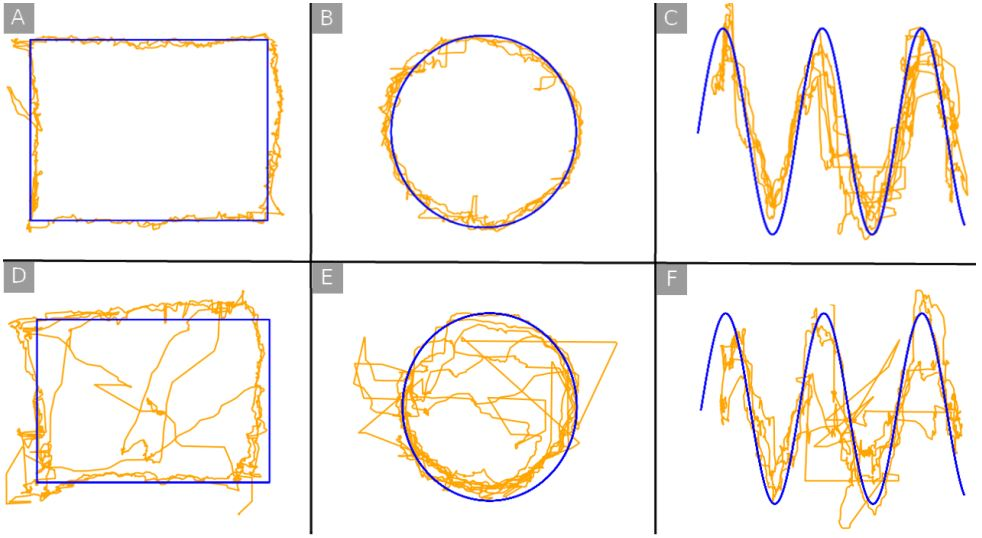
\includegraphics[width=0.7\linewidth]{figures/Smooth_Pursuit}
	\caption[آزمایش دنبال کردن روان یک شیء]{خطوط آبی مسیری است که شیء متحرک روی آن حرکت کرده و خطوط نارنجی مسیر دنبال کردن روان چشم است. ردیف بالایی حالتی است که کاربر بارشناختی کمی داشته و ردیف پایین بار شناختی بالا}
	\label{fig:smoothpursuit}
\end{figure}


\subsection{معیار‌های سیگنال مغزی}
ای‌ای‌جی یک روش محبوب تصویر برداری عصبی
\LTRfootnote{Neuroimaging}
است و با استفاده از الکترود‌های قرار گرفته بر روی سر به اندازه‌گیری فعالیت های الکتریکی مغز می‌پردازد. سنجش به کمک دستگاه ای‌ای‌جی به دلیل ثبت لحظه‌ای و پیوسته سیگنال‌های مغزی و می‌تواند به خوبی نشان دهنده کوچکترین تغییرات در بارشناختی بر اثر انجام آزمایش‌های مختلف باشد، از این رو استفاده از آن بسیار امیدوار کننده است . در ادامه فرایند‌های ثبت و تحلیل و سپس معیار‌های استخراج شده از آن برای سنجش بار شناختی بررسی می‌شود.
\subsubsection{باندهای مختلف سیگنال مغزی}
با توجه به فرکانس‌های امواج مغز آن‌ها را به پنج دسته یا باند تقسیم کرده‌اند. در شکل
\ref{fig:this-frequency-bands-of-eeg-signal}
می‌توانید نمونه این پنج دسته را مشاهده کنید. از این میان دو باند به دشواری فعالیت گزارش شده‌اند، آلفا و تتا. معمولا چگالی طیف توان
\LTRfootnote{Power Spectral Density}
 هر باند محاسبه می‌شود و سپس از آن برای مطالعه آزمایش مورد نظر استفاده می‌شود.
 \\
 مغز انسان در حالات مختلف مانند بیداری، خواب و یا خشم فرکانس‌های متفاوتی از خود بروز می‌دهد همچنین ویژگی‌های این امواج با تغییر سن نیز تغییر می‌کنند. 
 در ادامه به صورت جداگانه به بررسی هریک از باند‌های مغز می‌پردازیم.
\begin{figure}[htbp]
	\centering
	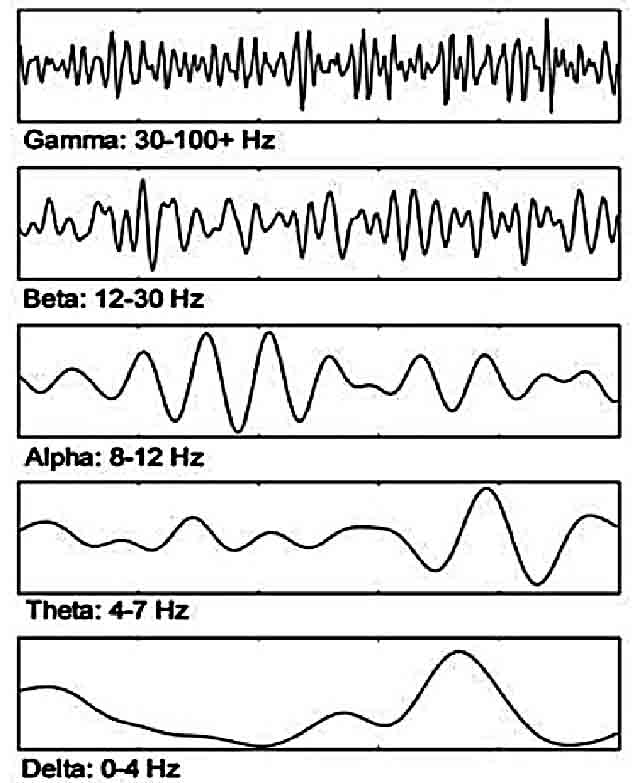
\includegraphics[width=0.5\linewidth]{figures/This-Frequency-bands-of-EEG-signal}
	\caption[باندهای امواج مغزی]{پنج باند فرکانس مغزی از بیشترین فرکانس در ردیف اول تا کمترین فرکانس در ردیف آخر نمایش داده شده‌است}
	\label{fig:this-frequency-bands-of-eeg-signal}
\end{figure}

\subsubsection*{امواج گاما - $ \gamma $}
فرکانس ریتم یا امواج گاما در محدوده بین ۳۰ تا ۱۰۰ هرتز قرار دارد. این امواج با ورودی‌های حسی و همچنین حافظه و توجه مرتبط هستند.
در برخی از تحقیقات، فعالیت‌های غیرمعمول در امواج گاما، برای بیماری‌هایی چون پارکینسون و صرع و آلزایمر گزارش شده‌است. همچنین در اختلال‌های خُلقی مثل افسردگی عمده و اختلال دوقطبی نیز دیده شده است.
\subsubsection*{امواج بتا - $ \beta $}
این امواج در فرکانس بین ۱۲ تا ۳۰ هرتز قرار دارند. باند بتا نمایانگر حالتی در مغز هستند که در هوشیاری معمول اتفاق می‌افتند. در فعالیت‌هایی مانند تفکر و یا توجه فعال، تمرکز، حل مسئله در بزرگسالان نرمال وجود دارد. این امواج در نواحی جلویی و مرکزی مغز وجود دارند، سطح بالای آن می‌تواند نشان دهنده وحشت باشد.
\subsubsection*{امواج آلفا - $ \alpha $}
معمولا فرکانس این امواج در ناحیه ۸ تا ۱۲ هرتز قرار دارد. این امواج معمولا با بسته شدن چشم‌ها در حالت استراحت، آرامش و خواب سبک ظاهر می‌شوند و در حالت خواب عمیق و یا اضطراب از بین می‌روند. میان افراد خلاق و سایرین در این ریتم تفاوت دیده شده است؛ به نحوی که در هنگام حل یک مسئله جدید هستند و ایده جدیدی دارند در نیمکره چپ مغز خود امواج آلفای بیشتری نسبت به بقیه تولید می‌کنند. این امواج معمولا در قسمت آکسیپیتال ظاهر می‌شوند.
\subsubsection*{امواج تتا - $ \theta $}
عموما این امواج در فرکانس ۴ تا ۷ هرتز قرار دارند. این امواج معمولا در هنگامی که هوشیاری به سمت خواب‌آلودگی می‌رود ظاهر می‌شوند. این امواج به سادگی در قسمت هیپوکمپوس
\LTRfootnote{hippocampus}
مشاهده می‌شوند البته ممکن است در سایر نواحی با احساسات مختلف نیز ظاهر شوند. در آزمایش‌هایی که حافظه کوتاه مدت را مورد بررسی قرار می‌دهند نیز دیده شده است.
\cite{vertes2005hippocampal}

\subsubsection*{امواج دلتا- $ \delta $}
 امواج دلتا در محدوده بیشتر از صفر  تا ۴ هرتز قرار می‌گیرند. این ریتم را به حالت خواب عمیق و آرام نسبت داده‌اند. ممکن است با نویز امواجی که از حرکت عضلات فک و گردن تولید می‌شوند اشتباه گرفته شود که البته به کمک نرم‌افزار‌های پردازش داده‌های مغزی میتوان آن‌ها را از یکدیگر تمیز داد. در بیماری‌های چون اسکیزوفرنی و پارکینسون نیز ظهور این امواج دیده شده است.
\subsubsection{استفاده از تغییرات، بجای قدرت سیگنال}
در پژوهش‌هایی که از داده‌های ‌ای‌ای‌جی استفاده می‌کنند معمولا از تغییرات سیگنال حاصل شده از یک کار یا فعالیت خاص بجای قدر مطلق قدرت
\LTRfootnote{Absolute power}
آن سیگنال استفاده می‌کنند. دلیل این امر آن است که مشاهدات نشان داده اند رفتار امواج مغزی با توجه به تفاوت‌های فردی، حجم مغز و سن افراد تفاوت پیدا می‌کند. از این رو از معیار
\lr{event related de-synchronization}
یا به اختصار
\lr{ERD/ERS}
استفاده می‌کنند.
معمولا در آزمایش و فعالیت های پژوهشی که داده مغزی گرفته می‌شود حاتی را نیز در نظر می‌گیرند که از او هیچ کاری نمیخواهند و فعالیتی انجام نمی‌دهد به این حالت باز پایه یا مرجع
\LTRfootnote{Baseline}
 می‌گویند.
 \\
 ERD/ERS
 طبق رابطه 
 \ref{eq:ERD-ERS}
 تعریف می‌شود.
 \begin{equation}\label{eq:ERD-ERS}
 \text{ERD/ERS}\% = \dfrac{\text{baseline interval band power - test interval band power}}{\text{baseline interval band power}}\times 100
 \end{equation}
 رابطه 
 \ref{eq:ERD-ERS}
را می‌توان اینگونه توضیح داد که 
ERD/ERS
نشان دهنده درصد افزایش یا کاهش قدرت باند در طول بازه مد نظر نسبت به بازه‌ی پایه.
این شاخص برای دو باند آلفا و تتا در بسیاری از آزمایش‌های شناختی حساس نسبت به سطح دشواری کار است.
\subsection{مزایا و معایب استفاده از سیگنال‌های مغزی}
\label{bbc:eeg_procon}
\paragraph{نقاط قوت}
اکثر روش‌های ثبت و سنجش فعالیت های مغزی یا نیازمند تجهیزات گران قیمت و پیشرفته که جهت کار با آنها نیاز به دانش پزشکی هستند و یا کار با آن‌ها برای آزمایش‌دهنده آسان نیست. همانند برش‌نگاری با گسیل پوزیترون
\LTRfootnote{Positron Emission Tomography - PET scan}
که نیازمند خوردن مواد خطرناک توسط آزمایش دهنده هستند یا دستگاه fMRI که فرد باید در حالت دراز کشیده بدون حرکت باشد، با این حال دستگاه‌های ثبت سیگنال مغزی بسیار کوچک‌‌تر و حتی نسخه‌های قابل حمل آن نیز موجود می‌باشد و تنها نیازمند به شرایط  معمول آزمایش‌گاهی است.
\\
ثبت سیگنال مغزی به وسیله ای‌ای‌جی از دقت زمانی بسیار خوبی (میلی‌ثانیه) بهره می‌برد از این رو میتوان به صورت پیوسته کوچک‌ترین مداخلات شناختی را شناسایی و اندازه‌گیری کرد.
\\
نرم‌افزار های قدرتمندی که در کنار این دستگاه‌ها استفاده می‌شوند توانایی خوبی در حذف و فیلتر کردن اثرات ناخواسته و یا نویز‌ها را دارند.
\paragraph{نقاط ضعف}
داده‌های
EEG
از دقت مکانی کمی برخوردار هستند (حدود سانتی متر) از این رو نمی‌توان به طور دقیق مکان فعالیت‌های مغزی را ثبت نمود. یکی دیگر از ضعف‌های داده‌های 
EEG
 نویز پذیر بودن آن است، این سیگنال‌ها می‌توانند به راحتی توسط حرکاتی چون: پلک زدن، نفس کشیدن، ضربان قلب، فرو بردن آب دهان و یا تکان خوردن سر تحت تاثیر قرار بگیرند که گاها این سیگنال‌ها از فعالیت‌های عصبی قوی‌تر هستند.
 \cite{antonenko2010using}
\subsection{ثبت سیگنال مغزی}
همان گونه که در شکل
\ref{fig:fnhum-05-00089-g002}
مشاهده می‌کنید اجزا تشکیل دهنده دستگاه ثبت سیگنال مغزی از سه قسمت تقویت کننده، ذخیره کننده و نمایش دهند سیگنال ها تشکیل شده است.
\begin{figure}[htbp]
	\centering
	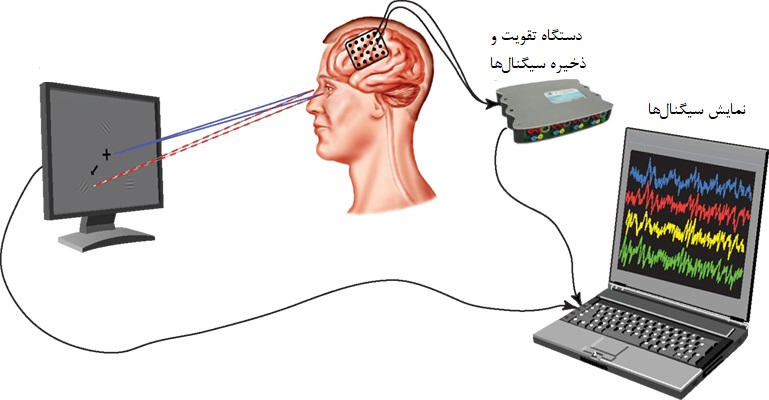
\includegraphics[width=0.9\linewidth]{figures/fnhum-05-00089-g002}
	\caption[اجزا دستگاه ثبت سیگنال مغزی]{حسگر‌ها داده‌های فعالیت های الکتریکی مغز را به تقویت کننده و ذخیره کننده سیگنال‌ها می‌فرستند و سپس توسط سیستم به نمایش در می‌آیند.}
	\label{fig:fnhum-05-00089-g002}
\end{figure}
\\
وجود بافت‌های ضخیمی مثل، استخوان، ماهیچه و خون در مسیر عبور سیگنال‌های مغزی  از محل تولید آن در قشر مغز تا محل قرارگیری الکترود‌های گیرنده، اندازه این سیگنال‌ها به شدت ضعیف می‌شوند از این رو جهت قابل مشاهده و استفاده بودن آن‌ها از تقویت کننده‌هایی برای تقویت آن‌ها استفاده می‌شود.
\cite{kheradpisheh2014evidence}
جهت ثبت با کیفیت بهتر سیگنال‌های مغزی میزان اتصال آن‌ها با پوست سر اهمیت دارد از این رو از ژل های مخصوصی جهت رسانایی بیشتر استفاده می‌شود.
\\
به جهت امکان مقایسه نتایج داده‌های EEG پژوهشگران، استانداردی تحت عنوان ۱۰-۲۰ که مکان الکترودها را روی قشر‌های مختلف مغز مشخص می‌کند ایجاد شده است. عددهای ۱۰ و ۲۰ در نام این روش، بیانگر این موضوع هستند که فاصله بین دو الکترود متوالی، همواره برابر با ۱۰٪ یا ۲۰٪ اندازه فاصله جلو-عقب سر یا فاصله راست تا چپ سر است. در این حالت تعداد الکترود‌های به کار رفته ۲۱ عدد است در برخی کاربرد‌ها تعداد بیشتر الکترود نیز ممکن است.
\\
در این روش مکان هر الکترود با دو کاراکتر مشخص می‌شود.

کاراکتر نخست، که یک حرف انگلیسی است، بیانگر قسمتی از نواحی مغز است که الکترود روی آن قرار می‌گیرد و کاراکتر بعدی که یک عدد است، بیانگر نیم کره راست و چپ مغز است. در جدول
\ref{tab:EEG_CHAR}
نمادها و معنای آن‌ها را می‌بینید.
\begin{center}
	\begin{table}[h]
	\centering
	\caption{نمادهای استفاده شده در استاندارد ۱۰-۲۰ التروانسفالوگرافی}
	\label{tab:EEG_CHAR}
	\begin{tabular}{|c|c|c|c|c|c|c|c|c|}
		\hline
		اعداد فرد    & اعداد زوج  & z      & O      & P         & C     & T        & F      &\textbf{ نماد}      \\ \hline
		نیم کره راست & نیم کره چپ & فرق سر & پس‌سری & آهیانه‌ای & مرکزی & گیج‌گاهی & پیشانی & \textbf{ناحیه مغز} \\ \hline
	\end{tabular}
\end{table}
\end{center}
در شکل
\ref{fig:LOB_1020}
محل قرارگیری الکترودها و لو‌ب‌های مغز را می‌بینید.
به جهت پرهیز از اندازه‌گیری های وقت‌گیر و دقت بیشتر در اندازه‌گیری سیگنال‌های مغزی الکترود ها را مطابق استاندارد ۱۰-۲۰ می‌توان بر روی یک کلاه  قرار داد، در این صورت با قرار دادن کلاه بر روی سر خودبه‌خود الکترود ها در مکان مناسب قرار می‌گیرند. نمونه‌ای از آن را در شکل 
\ref{fig:eegcap}
می‌بینید.
\begin{figure}[htbp]
	\centering
	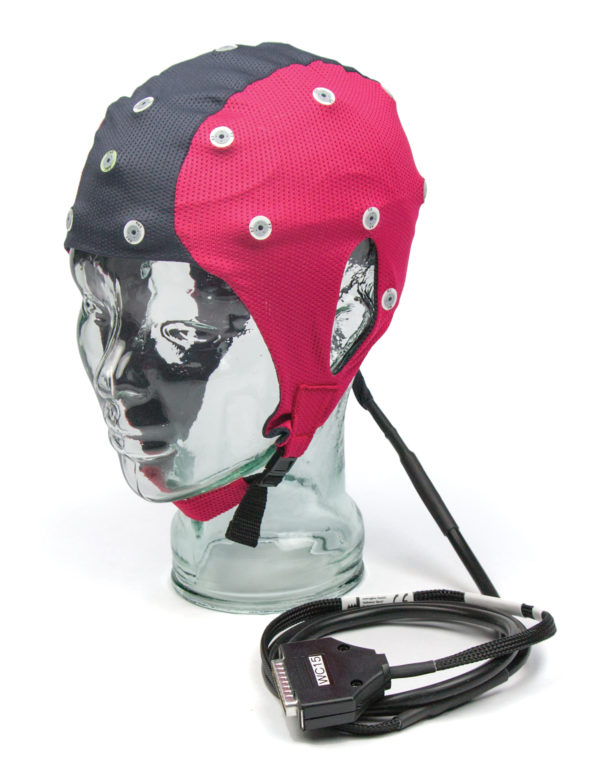
\includegraphics[width=0.3\linewidth]{figures/EEG_cap}
	\caption[کلاه ثبت سیگنال مغزی]{استفاده از کلاه ثبت سیگنال مغزی به منظور اندازه‌گیری دقیق و ساده‌تر}
	\label{fig:eegcap}
\end{figure}

\begin{figure}[htbp]
	\centering
	\begin{subfigure}{\textwidth}
		\centering
		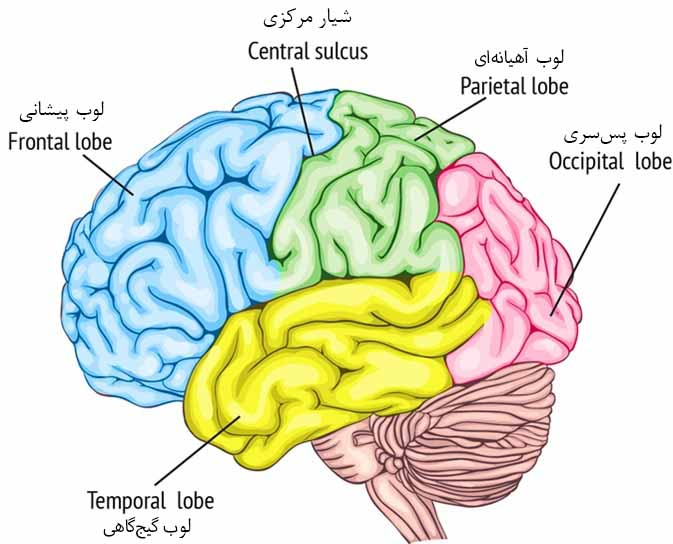
\includegraphics[width=.7\linewidth]{figures/brain_lobes}
		\caption{طرحی از مغز و چهار لوب آن}
		\label{fig:brainlobes}
	\end{subfigure}
	\begin{subfigure}{\textwidth}
		\centering
		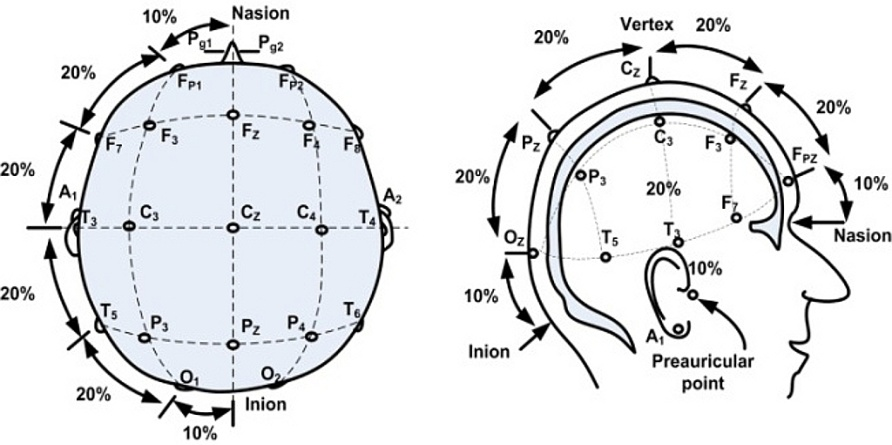
\includegraphics[width=\linewidth]{figures/EEG_10-20}
		\caption{نقاط قرارگیری الکترود‌های دستگاه الکتروانسافلوگراف بر روی سر مطابق استاندارد ۱۰-۲۰}
		\label{fig:eeg10-20}
	\end{subfigure}
	\caption[لوب‌های مغز و استاندارد ۱۰-۲۰]{مکان قرارگیری الکتوردهای دستگاه الکتروانسافلوگراف و لوب‌های مغز}
	\label{fig:LOB_1020}
\end{figure}

